\documentclass{beamer}
%Information to be included in the title page:
\title{Domača naloga 1}
\author{Ambrož Tacar}
\institute{Fakulteta za strojništvo,UL}
\date{2024}
\begin{document}
\frame{\titlepage}
\begin{frame}
\frametitle{Kazalo vsebine}
\tableofcontents
\end{frame}
\begin{frame} 
\section{Vsebina datoteke $naloga1\_1.txt$}
\frametitle{Vsebina datoteke $naloga1\_1.txt$}
Tekstovna datoteka vsebuje vrednosti časa in nekaj drugih informacij. Vsebina posameznih vrstic datoteke pa je sledeča:
\begin{itemize}
    \item prva vrstica: ime količine, ki jo podatki predstavljajo ($time[s]$)
    \item druga vrstica: število preostalih vrstic (100) in število podatkov v posameznih preostalih vrsticah (1)
    \item ostale vrstice: vrednosti časa
\end{itemize}
\vspace{5pt}
\textbf Za branje podatkov sem uporabil funkcijo $importdata(vhodni\ podatki).data()$ :
\begin{itemize}
    \item vhodni podatki: $(ime\ datoteke,\ delilni\ znak,\ število\ izpuščenih\ začetnih\ vrstic)$ 
    \item izhodni podatki: numerično polje/ matrika/ vektor 
\end{itemize}
\end{frame}
\begin{frame} 
\section{Graf $P(t)$}
\frametitle{Graf $P(t)$}
Na podlagi vrednosti, pridobljenih iz obeh tekstovnih datotek, sem s funkcijo $plot$ izrisal graf moči v odvisnosti od časa (P(t)) in mu dodal naslov, označil osi in prilagodil območje, ki ga graf prikazuje.
\begin{figure}
    \centering
    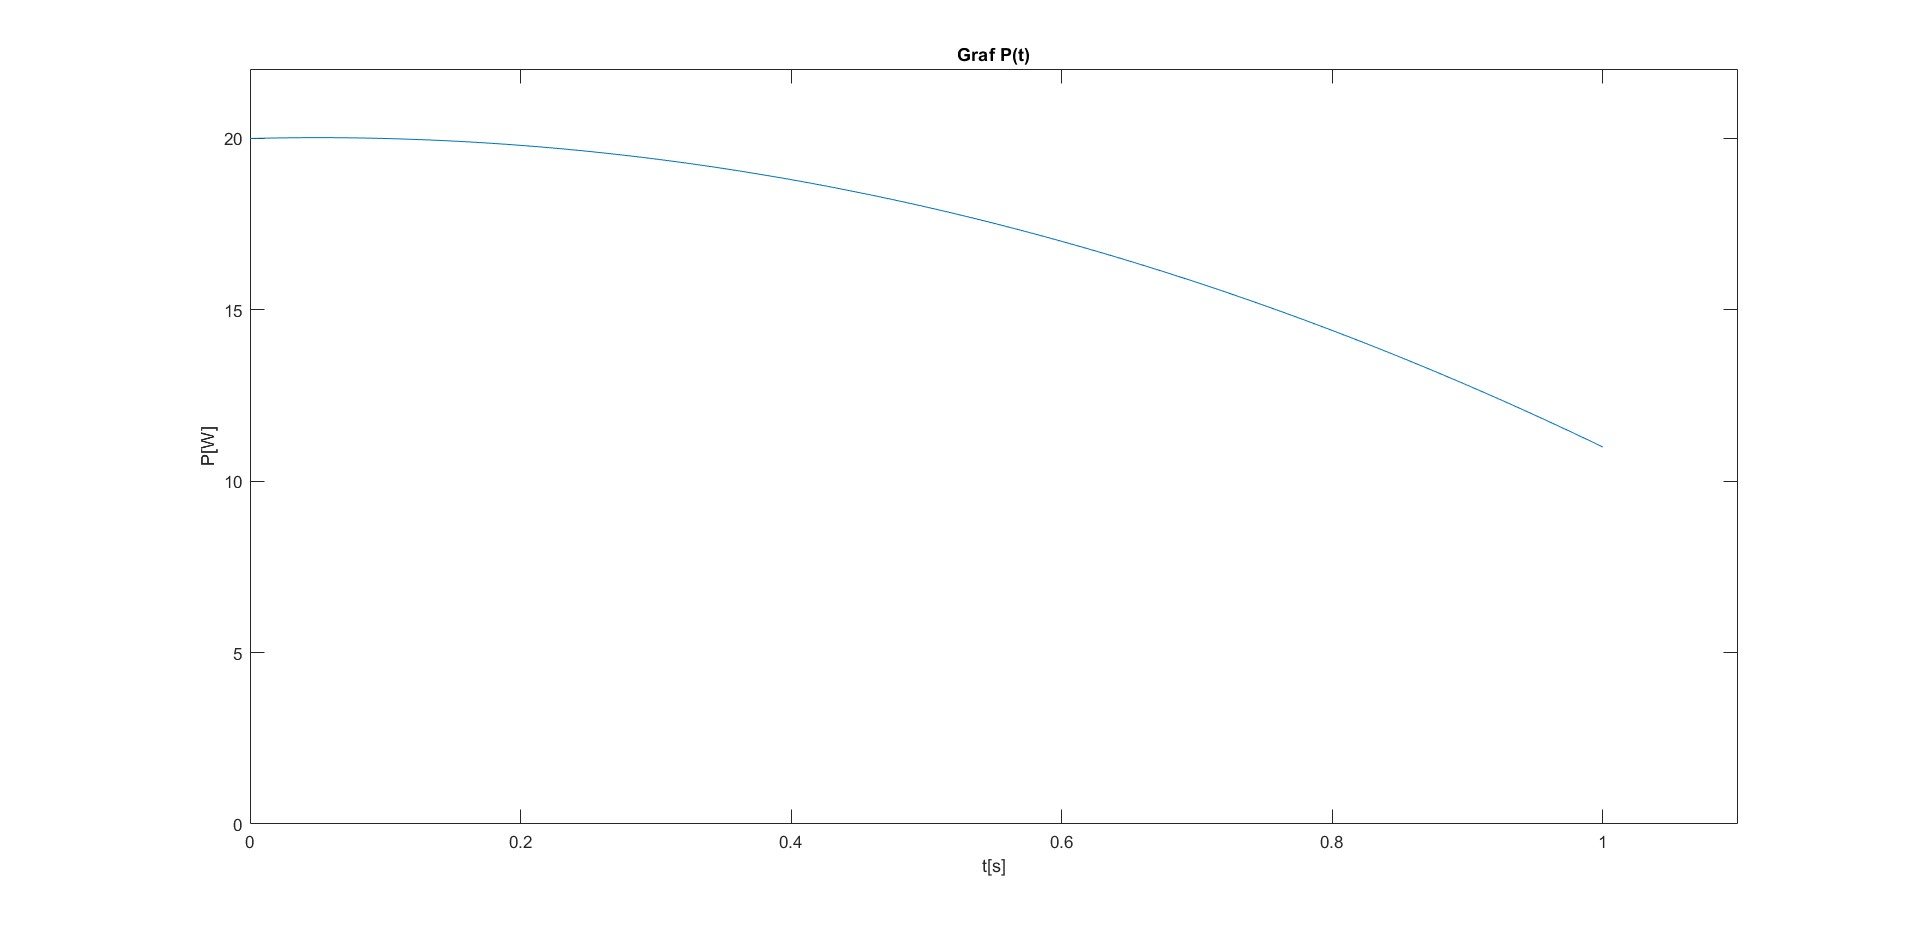
\includegraphics[width=0.9\linewidth]{Graf P(t).jpg}
    \label{P(t)}
\end{figure}
\end{frame} 
\section{Trapezna metoda}
\begin{frame}[fragile]
\frametitle{Trapezna metoda}
Za izračun integrala $$\int_{t_{min}}^{t_{max}} P(t)dt\ ,$$sem uporabil trapezno formulo:
$$\sum_{i=1}^{n-1} \frac{\Delta t_i}{2} (P_i + P_{i+1})\ ,$$
kjer $n$ predstavlja število podatkov, $P_i$ posamezno vrednost moči in $\Delta t_i$ časovni korak ($\Delta t_i = t_{i+1} - t_i$). 
Zgornjo formulo sem v MATLABU-u zapisal s pomočjo $for$ zanke in za rezultat dobil $17.1665\ J$, ki za $7.1054\times 10^{-15}\ J$ odstopa od rezulata, dobljenega z vgrajeno fukcijo $trapz$.
\end{frame}
\end{document}